%==============================================================================
% Chapitre 52 - Les munitions spéciales
%==============================================================================

\section{Introduction}

Toutes les munitions ne sont pas destinées à produire un simple effet de
perforation ou de neutralisation.

Au fil du temps, de nombreuses munitions spécialisées ont été développées afin
de répondre à des besoins particuliers.

Ces munitions peuvent être destinées :

\begin{itemize}
    \item à l'entraînement ;
    \item au réglage du tir ;
    \item à la signalisation ;
    \item à la simulation ;
    \item à certaines applications techniques.
\end{itemize}

\begin{aretenir}

Une munition spéciale est conçue pour remplir une fonction particulière qui
dépasse le simple tir conventionnel.

\end{aretenir}

\section{Diversité des munitions spéciales}

Les munitions spéciales regroupent une famille très vaste.

On y trouve notamment :

\begin{itemize}
    \item les cartouches à blanc ;
    \item les cartouches d'exercice ;
    \item les munitions traçantes ;
    \item les munitions de signalisation ;
    \item les munitions de réglage ;
    \item les munitions non létales.
\end{itemize}

\begin{figure}[htbp]
\centering

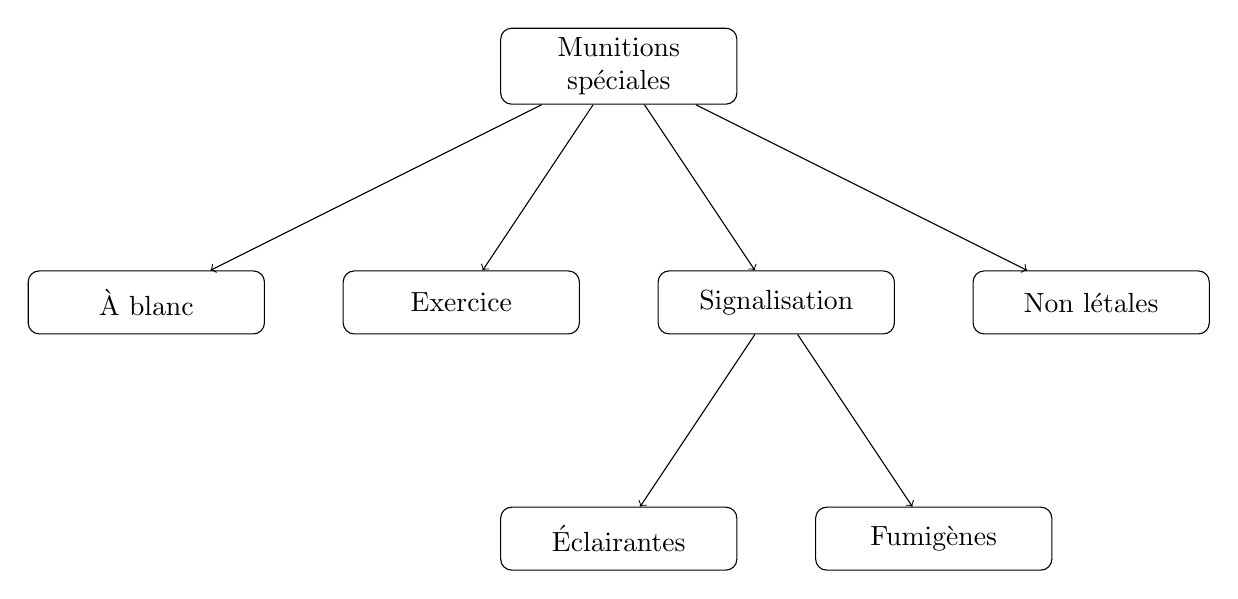
\begin{tikzpicture}[
every node/.style={
draw,
rounded corners,
align=center,
minimum width=3cm,
minimum height=8mm
}
]

\node (M) at (0,0) {Munitions\\spéciales};

\node (B) at (-6,-3) {À blanc};
\node (E) at (-2,-3) {Exercice};
\node (S) at (2,-3) {Signalisation};
\node (N) at (6,-3) {Non létales};

\draw[->] (M) -- (B);
\draw[->] (M) -- (E);
\draw[->] (M) -- (S);
\draw[->] (M) -- (N);

\node (Ec) at (0,-6) {Éclairantes};
\node (Fu) at (4,-6) {Fumigènes};

\draw[->] (S) -- (Ec);
\draw[->] (S) -- (Fu);

\end{tikzpicture}

\caption{Exemple simplifié de classification des munitions spéciales.}
\label{fig:munitions_speciales}

\end{figure}

\section{Cartouches à blanc}

Les cartouches à blanc ne propulsent généralement pas de projectile.

Elles produisent néanmoins :

\begin{itemize}
    \item du bruit ;
    \item une flamme de bouche ;
    \item des gaz sous pression.
\end{itemize}

Elles sont largement utilisées pour l'instruction et les cérémonies.

\begin{figure}[htbp]
\centering

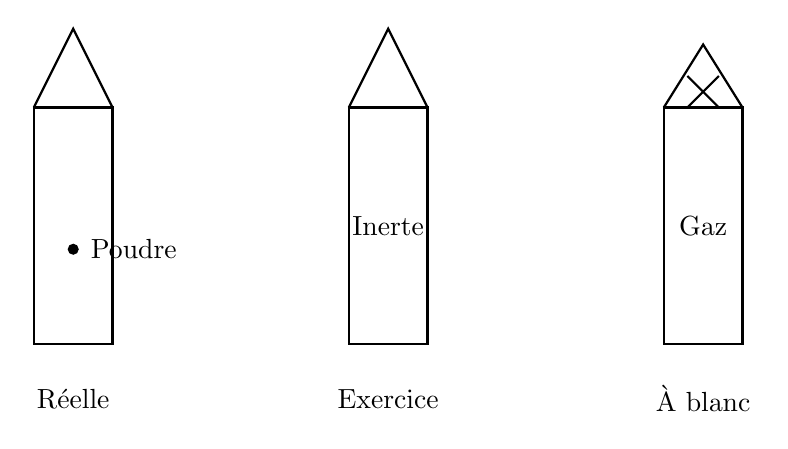
\begin{tikzpicture}[scale=1]

% Réelle
\begin{scope}

\draw[thick] (0,0) rectangle (1,3);
\draw[thick] (0,3) -- (0.5,4) -- (1,3);

\node at (0.5,-0.7) {Réelle};

\fill (0.5,1.2) circle (2pt);
\node[right] at (0.6,1.2) {Poudre};

\end{scope}

% Exercice
\begin{scope}[xshift=4cm]

\draw[thick] (0,0) rectangle (1,3);
\draw[thick] (0,3) -- (0.5,4) -- (1,3);

\node at (0.5,-0.7) {Exercice};

\node at (0.5,1.5) {Inerte};

\end{scope}

% Blanc
\begin{scope}[xshift=8cm]

\draw[thick] (0,0) rectangle (1,3);

\draw[thick]
(0,3)
--
(0.5,3.8)
--
(1,3);

\draw[thick]
(0.3,3.4)
--
(0.7,3.0);

\draw[thick]
(0.3,3.0)
--
(0.7,3.4);

\node at (0.5,-0.7) {À blanc};

\node at (0.5,1.5) {Gaz};

\end{scope}

\end{tikzpicture}

\caption{Comparaison simplifiée entre une cartouche réelle, une cartouche d'exercice et une cartouche à blanc.}
\label{fig:types_cartouches}

\end{figure}

\section{Risques associés}

L'absence de projectile ne signifie pas l'absence de danger.

Les gaz expulsés à la bouche peuvent provoquer des blessures à courte
distance.

Des règles de sécurité spécifiques doivent être appliquées.

\section{Cartouches d'exercice}

Les cartouches d'exercice reproduisent généralement :

\begin{itemize}
    \item les dimensions ;
    \item la masse ;
    \item l'encombrement ;
    \item le fonctionnement mécanique.
\end{itemize}

Elles permettent l'entraînement sans tir réel.

\section{Cartouches inertes}

Certaines cartouches sont totalement inertes.

Elles ne contiennent :

\begin{itemize}
    \item ni amorce active ;
    \item ni poudre ;
    \item ni composition pyrotechnique.
\end{itemize}

Elles servent principalement à l'instruction.

\section{Munitions de signalisation}

Certaines munitions sont destinées à transmettre une information visuelle.

Elles peuvent produire :

\begin{itemize}
    \item une lumière ;
    \item une couleur ;
    \item un signal visible à grande distance.
\end{itemize}

\section{Munitions éclairantes}

Les munitions éclairantes sont conçues pour illuminer temporairement une zone.

Elles sont utilisées :

\begin{itemize}
    \item pour l'observation ;
    \item pour la surveillance ;
    \item pour certaines opérations nocturnes.
\end{itemize}

\section{Munitions fumigènes}

Les munitions fumigènes produisent un nuage de fumée.

Celui-ci peut servir :

\begin{itemize}
    \item au marquage ;
    \item à la signalisation ;
    \item au camouflage.
\end{itemize}

\section{Munitions de réglage}

Certaines munitions permettent d'observer plus facilement l'impact ou la
trajectoire.

Elles facilitent :

\begin{itemize}
    \item le réglage des armes ;
    \item le contrôle des tirs ;
    \item l'entraînement.
\end{itemize}

\section{Munitions non létales}

Certaines applications nécessitent de limiter les effets produits.

Les munitions dites non létales cherchent à réduire le risque de blessures
graves tout en conservant un effet incapacitant.

\section{Limites du terme non létal}

L'expression \emph{non létal} peut être trompeuse.

Toute munition capable de transmettre une quantité suffisante d'énergie peut
présenter un danger.

C'est pourquoi l'expression :

\begin{quote}
à létalité réduite
\end{quote}

est parfois préférée.

\section{Applications policières}

Les forces de l'ordre utilisent diverses munitions spécialisées.

Leur objectif peut être :

\begin{itemize}
    \item le maintien de l'ordre ;
    \item la neutralisation temporaire ;
    \item la dispersion ;
    \item l'interpellation.
\end{itemize}

\section{Applications industrielles}

Certaines munitions sont utilisées en dehors du domaine militaire ou sportif.

On peut citer notamment :

\begin{itemize}
    \item les outils de scellement ;
    \item certaines applications pyrotechniques ;
    \item certains dispositifs de sécurité.
\end{itemize}

\section{Contraintes réglementaires}

Les munitions spéciales sont souvent soumises à des réglementations
particulières.

Ces règles varient selon :

\begin{itemize}
    \item les pays ;
    \item les usages ;
    \item les catégories de munitions.
\end{itemize}

\section{Pourquoi autant de variantes ?}

Chaque mission impose des contraintes spécifiques.

Une munition optimisée pour l'éclairage ne peut pas remplir efficacement une
fonction de signalisation ou d'entraînement.

Cette spécialisation explique la grande diversité observée.

\begin{figure}[htbp]
\centering

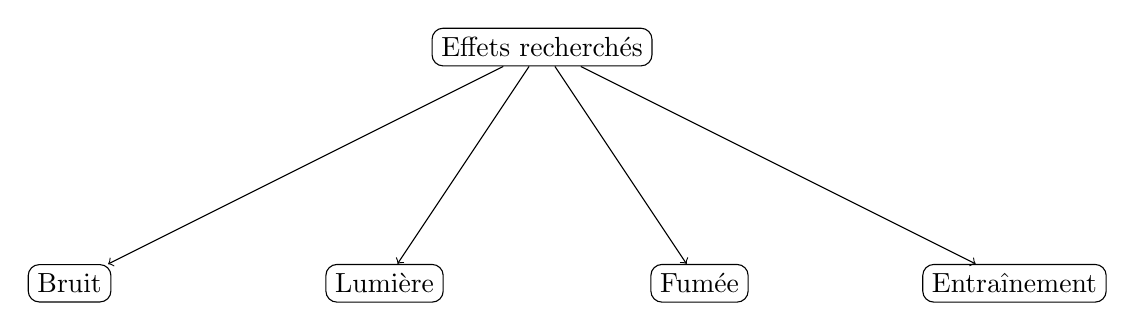
\begin{tikzpicture}[scale=1]

\node[draw,rounded corners]
(M)
at (0,0)
{Effets recherchés};

\node[draw,rounded corners]
(B)
at (-6,-3)
{Bruit};

\node[draw,rounded corners]
(L)
at (-2,-3)
{Lumière};

\node[draw,rounded corners]
(F)
at (2,-3)
{Fumée};

\node[draw,rounded corners]
(E)
at (6,-3)
{Entraînement};

\draw[->] (M) -- (B);
\draw[->] (M) -- (L);
\draw[->] (M) -- (F);
\draw[->] (M) -- (E);

\end{tikzpicture}

\caption{Exemples d'effets recherchés avec les munitions spéciales.}
\label{fig:effets_munitions_speciales}

\end{figure}

\section{Vers les munitions de chasse}

Les munitions spéciales illustrent la capacité d'adaptation des technologies
balistiques.

Nous allons maintenant revenir à un domaine majeur du monde civil : les
munitions de chasse.

\section{À retenir}

\begin{aretenir}

\begin{itemize}
    \item Les munitions spéciales répondent à des besoins particuliers.
    \item Les cartouches à blanc et les cartouches d'exercice sont largement
          utilisées pour l'instruction.
    \item Les munitions de signalisation remplissent des fonctions
          d'information et de repérage.
    \item Les munitions non létales restent potentiellement dangereuses.
    \item La spécialisation des usages explique la grande diversité des
          conceptions.
\end{itemize}

\end{aretenir}
